\chapter{ARM M4}
The ARM M4 MCU is the base of the stm32f407. ARM offers the IP of the
CORE-M4 to manufacturers and they can customize the IP as they demand.
A very simple diagram of the used MCU is the following:\\

\begin{figure}[ht]
	\centering
	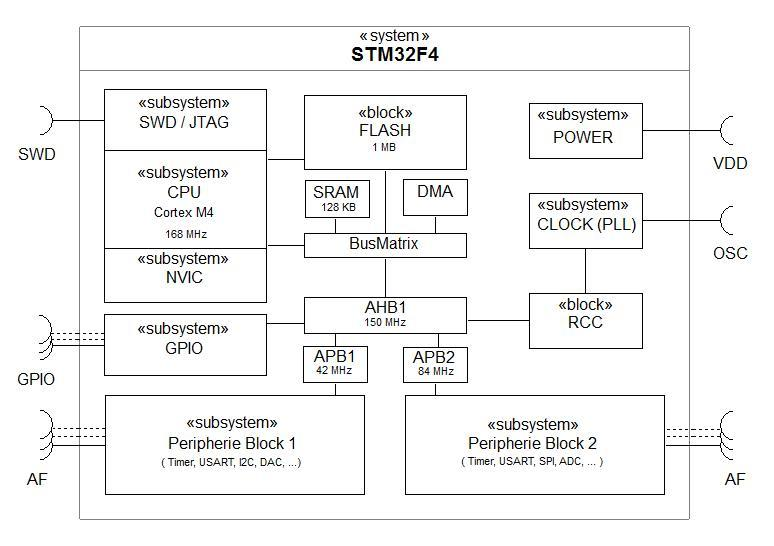
\includegraphics[width=400px,height=300px]{../img/stm32f4_prinzip.jpeg}
	\caption{Simple M4 Diagram}
	\label{m4_simple}
\end{figure}

The diagram doesn't show, which peripherie systems are connected to which
APBX-Bus, but that can be seen in the datasheet. What it does show is, that
the GPIO-Pins, are connected to the AHB1-Bus.\\
The reason for that is, that it's much faster what is recommended
 for most demands of GPIO. The subsystems on the other hand aren't
 necessarly needed to react that fast.\\

For example the USART6, which is used in the project, is connected to APB2.
A much more precise representation of the STM32F4 is following diagram.\\

The AHB1 is the system bus and therefore should be really fast.
\includepdf[pages={18}]{../img/blockdia.pdf}
